\addtocontents{toc}{\setcounter{tocdepth}{3}}
\chapter{Release 2 Administration et visualisation}

\section*{Introduction}
Ce chapitre fait l'objet d'une description du deuxième release du projet qui est la réalisation de
module d'administration (authentification et gestion des utilisateurs) et de visualisation (tableau de bord).\\
Il est constitué de deux sprints, à savoir le sprint 3 : authentification et gestion des utilisateurs et le sprint 4 : Visualisation de tableau de bord.\\
L'étude de chaque sprint couvre l'analyse, la conception, la réalisation et les tests fonctionnels.
\section{Sprint 3 Authentification et gestion des utilisateurs}
Ce sprint a pour but de développer les parties d'authentification et de gestion des utilisateurs.
\subsection{Backlog du Sprint}
Dans cette partie, nous allons présenter à travers le tableau 5.1 les différents user story pour le sprint 3.
\captionof{table}{Backlog du Sprint 3}

\begin{tabular}{@{}| >{\centering\arraybackslash}p{.04\textwidth}| >{\centering\arraybackslash}p{.30\textwidth}|>{\centering\arraybackslash}p{.06\textwidth}| >{\centering\arraybackslash}p{.35\textwidth}| >{\centering\arraybackslash}p{.13\textwidth}|@{}}

\hline \rowcolor{lightgray} \textbf{ID}  &  \textbf { User Story} & \textbf {ID Tâche} & \textbf {Tâche} & \textbf{Estimation (jours)} \\



\hline

\multirow{4}{*}{15} & \multirow{4}{.30\textwidth}{En tant qu’utilisateur, je dois
m’authentifier pour accéder à
l’application.}  & 15.1 
  & Implémenter le service AuthService. & 3 \\ 
\cline{3-5}
& &  15.2 & Implémenter les méthodes nécessaires pour
l’authentification. & 1 \\
\cline{3-5}
& &  15.3 & Préparer l’interface d’authentification. & 1 \\
\cline{3-5}
& &  15.4 & Tester l’authentification. & 1 \\


\hline

\multirow{4}{*}{16} & \multirow{4}{.30\textwidth}{En tant qu’administrateur, je veux
ajouter un utilisateur.}  & 16.1 
  & Implémenter les méthodes nécessaires pour
l’ajout.  & 1 \\ 
\cline{3-5}
& &  16.2 & Préparer l'interface graphique. & 1 \\
\cline{3-5}
& &  16.3 & Tester l'ajout d'un compte utilisateur. & 1 \\
\cline{3-5}





\hline
\end{tabular}



\begin{tabular}{@{}| >{\centering\arraybackslash}p{.04\textwidth}| >{\centering\arraybackslash}p{.30\textwidth}|>{\centering\arraybackslash}p{.06\textwidth}| >{\centering\arraybackslash}p{.35\textwidth}| >{\centering\arraybackslash}p{.13\textwidth}|@{}}

\hline \rowcolor{lightgray} \textbf{ID}  &  \textbf { User Story} & \textbf {ID Tâche} & \textbf {Tâche} & \textbf{Estimation (jours)} \\



\hline

\multirow{4}{*}{17} & \multirow{4}{.30\textwidth}{En tant qu’administrateur, je veux
modifier un utilisateur.}  & 17.1 
  & Implémenter les méthodes nécessaires pour
la modification.  & 1 \\ 
\cline{3-5}
& &  17.2 & Préparer l'interface graphique. & 1 \\
\cline{3-5}
& &  17.3 & Tester la modification d'un compte utilisateur. & 1 \\
\cline{3-5}


\hline

\multirow{4}{*}{18} & \multirow{4}{.30\textwidth}{En tant qu’administrateur, je veux
supprimer un utilisateur.}  & 18.1 
  & Implémenter les méthodes nécessaires pour
la suppression.  & 1 \\ 
\cline{3-5}
& &  18.2 & Tester la suppression d'un compte utilisateur. & 1 \\
\cline{3-5}
\hline

\multirow{4}{*}{19} & \multirow{4}{.30\textwidth}{En tant qu’administrateur, je
souhaite consulter et effectuer une
recherche sur la liste des utilisateurs.}  & 19.1 
  & Implémenter les méthodes nécessaires pour
la recherche et la consultation.  & 1 \\ 
\cline{3-5}
& &  19.2 & Préparer l'interface graphique. & 1 \\
\cline{3-5}
\hline

\multirow{4}{*}{20} & \multirow{4}{.30\textwidth}{En tant qu’administrateur, je
souhaite attribuer un rôle à un
utilisateur.}  & 20.1 
  & Implémenter les méthodes nécessaires pour
la gestion des rôles.  & 2 \\ 
\cline{3-5}
& &  20.2 & Préparer l'interface graphique. & 2 \\
\cline{3-5}
\hline
\end{tabular}


\subsection{Spécification fonctionnelle}
Le diagramme de la figure \ref{fig:release2sprint3} clarifie le fonctionnement de base d’un administrateur en gérant
les utilisateurs. Il doit s’authentifier pour pouvoir accéder à la gestion, il peut ajouter, modifier ou
supprimer un compte utilisateur.\\
La figure \ref{fig:release2sprint3} présente le cas d’utilisation détaillé de « Gérer les utilisateurs ».
\newpage
\begin{figure}[htpb]
    \centering
    \fcolorbox{brown}{white}{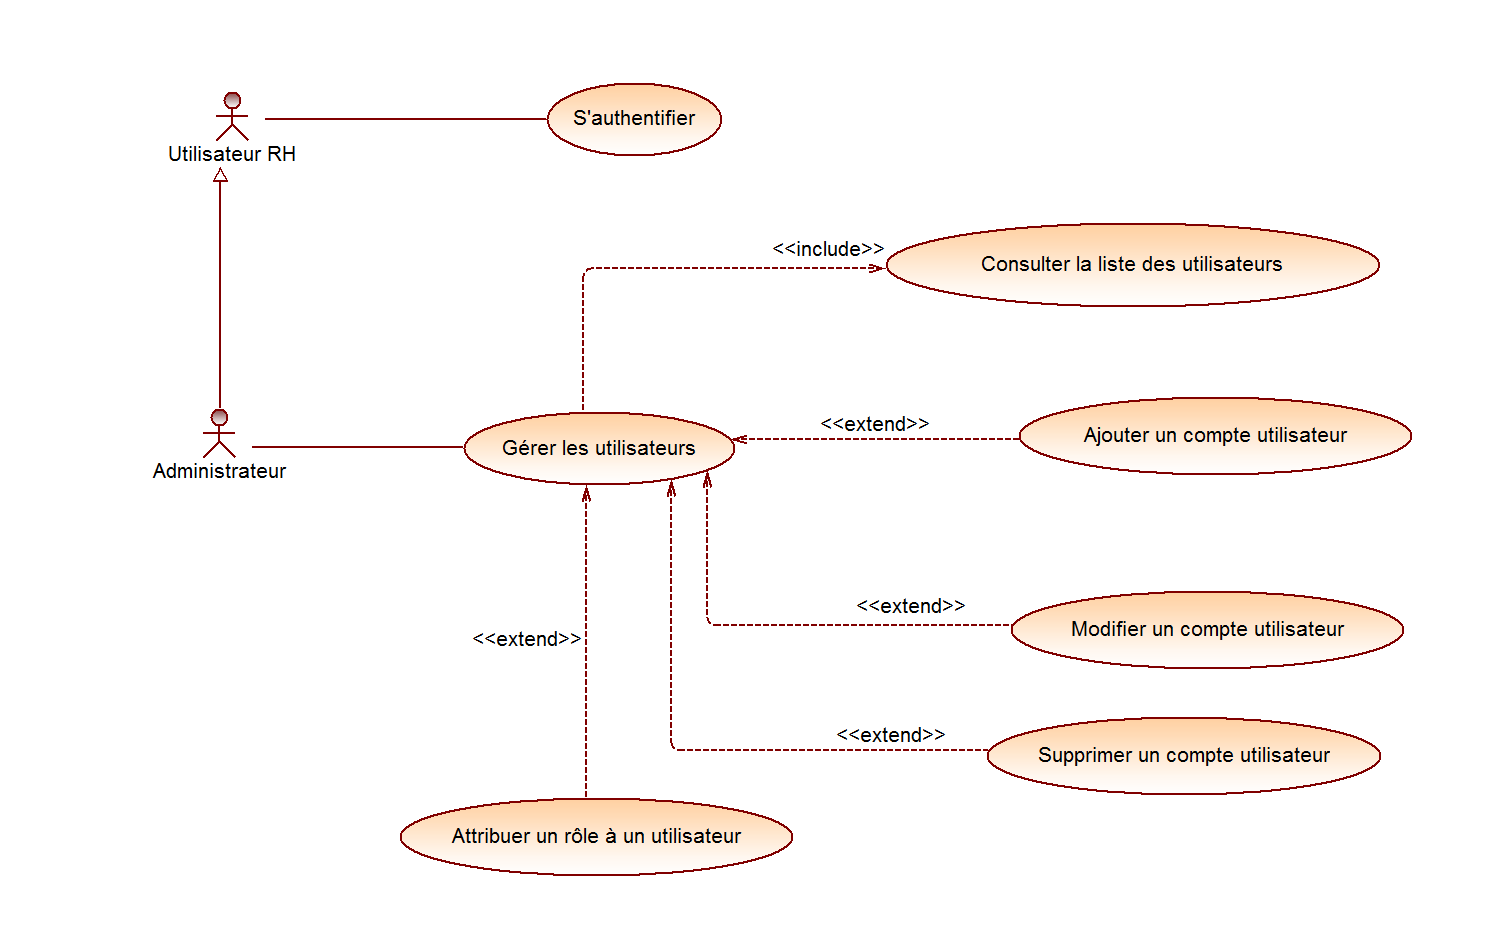
\includegraphics[width=1\linewidth]{img/release2sprint3_final.png}}
    \caption{Diagramme de cas d’utilisation « Gérer les utilisateurs »}
    \label{fig:release2sprint3}
    \end{figure}

    Le tableau \ref{tab:authentifierutilisateur} présente la description textuelle du cas d’utilisation «s'authentifier».
\begin{longtable}[c]{
    |p{.25\textwidth}
    |p{.71\textwidth}|
}
    \caption{Description du diagramme de cas d’utilisation <<s'authentifier>>}
    \label{tab:authentifierutilisateur}\\
    \hline
    
    Cas d’utilisation
    &  s'authentifier. \\
    \hline 
    
    Acteur
    & Administrateur, Utilisateur RH. \\
    \hline 
    
    Précondition
    & L’utilisateur doit saisir son code (« login») et son mot de passe. \\
    \hline
    
    Post-condition
    & L’utilisateur est authentifié. \\
    \hline
    
    Description du
scénario

    &      \begin{itemize}
    \item L’utilisateur accède à la page de l’authentification.
    \item L’utilisateur saisit son code (« login») et son mot de passe.
     \item L’application vérifie les coordonnées de l’utilisateur dans la base de données.
     \item L’application donne l’autorisation à l’utilisateur pour accéder à son propre espace de travail.
    \end{itemize}  \\
    \hline
    
   Cas alternatif
    & L’application renvoie l’utilisateur à la page de l’authentification suivie d’un message d’erreur.
 \\ \hline
   
\end{longtable}


    Le tableau \ref{tab:consulterCompteUtilisateur} présente la description textuelle du cas d’utilisation «Consulter la liste des utilisateurs».
\begin{longtable}[c]{
    |p{.25\textwidth}
    |p{.71\textwidth}|
}
    \caption{Description du diagramme de cas d’utilisation <<Consulter la liste des utilisateurs>>}
    \label{tab:consulterCompteUtilisateur}\\
    \hline
    
    Cas d’utilisation
    &  Consulter la liste des utilisateurs. \\
    \hline 
    
    Acteur
    & Administrateur. \\
    \hline 
    
    Précondition
    & L’administrateur s’est authentifié. \\
    \hline
    
    Post-condition
    &     \begin{itemize}
    \item Liste des utilisateurs affichée.
     \item Liste des utilisateurs filtrée.
    \end{itemize} \\
    \hline
    
    Description du
scénario

    &      \begin{itemize}
    \item L’administrateur choisit de consulter la liste des utilisateurs.
    \item Le système récupère la liste des utilisateurs.
     \item L’administrateur saisit le nom d'utilisateur pour filtrer la liste.
     \item Liste des utilisateurs filtrée s'affiche.
    \end{itemize}  \\
    \hline
    
   Exception
    & Erreur de connexion.
 \\ \hline
   
\end{longtable}

  Le tableau \ref{tab:ajouterCompteUtilisateurTab} présente la description textuelle du cas d’utilisation «Ajouter un compte utilisateur».
\begin{longtable}[c]{
    |p{.25\textwidth}
    |p{.71\textwidth}|
}
    \caption{Description du diagramme de cas d’utilisation <<Ajouter un compte utilisateur>>}
    \label{tab:ajouterCompteUtilisateurTab}\\
    \hline
    
    Cas d’utilisation
    &  Ajouter un compte utilisateur. \\
    \hline 
    
    Acteur
    & Administrateur. \\
    \hline 
    
    Précondition
    & L’administrateur s’est authentifié. \\
    \hline
    
    Post-condition
    & Compte utilisateur ajouté avec succès. \\
    \hline
    
    Description du
scénario

    &      \begin{itemize}
    \item L’administrateur choisit d’ajouter un nouveau compte utilisateur.
    \item Le système renvoie le formulaire d’ajout d’un compte utilisateur.
     \item L’administrateur remplit les champs nécessaires et valide la saisie.
     \item Le système vérifie les champs.
    \item Le système enregistre les données et affiche la liste des utilisateurs mise à jour.
    \end{itemize}  \\
    \hline
    
   Exception
    & Erreur de connexion.
 \\ \hline
   
\end{longtable}

 Le tableau \ref{tab:SupprimerCompteUtilisateur} présente la description textuelle du cas d’utilisation «Supprimer un compte utilisateur».
\begin{longtable}[c]{
    |p{.25\textwidth}
    |p{.71\textwidth}|
}
    \caption{Description du diagramme de cas d’utilisation <<Supprimer un compte utilisateur>>}
    \label{tab:SupprimerCompteUtilisateur}\\
    \hline
    
    Cas d’utilisation
    &  Supprimer un compte utilisateur. \\
    \hline 
    
    Acteur
    & Administrateur. \\
    \hline 
    
    Précondition
    & L’administrateur s’est authentifié. \\
    \hline
    
    Post-condition
    &     \begin{itemize}
    \item Compte utilisateur sélectionné est supprimé.
     \item Liste des utilisateurs affichée est mise à jour.
    \end{itemize} \\
    \hline
    
    Description du
scénario

    &      \begin{itemize}
    \item L’administrateur choisit un compte utilisateur à supprimer.
    \item Le système affiche un message de confirmation.
     \item L’administrateur confirme la suppression.
     \item Le système retourne la liste des utilisateurs mise à jour.
    \end{itemize}  \\
    \hline
    
   Exception
    & Erreur de connexion.
 \\ \hline
   
\end{longtable}
\newpage
\subsection{Conception}
\subsubsection{Diagramme de classes}
La figure \ref{fig:diagclasse3_new_3} définit les nouvelles classes utilisées en bleu pour le sprint 3.\\
Le contrôleur « UserController » joue le rôle d’intermédiaire entre l'entité « UserModel » et la
vue \newline « UserView » qui interagit avec l’utilisateur.
Au niveau du modèle, l’entité « UserModel » peut gérer plusieurs employés et l’entité «
EmployeeModel » est gérée par un seul utilisateur.
\begin{figure}[htpb]
    \centering
    \fcolorbox{brown}{white}{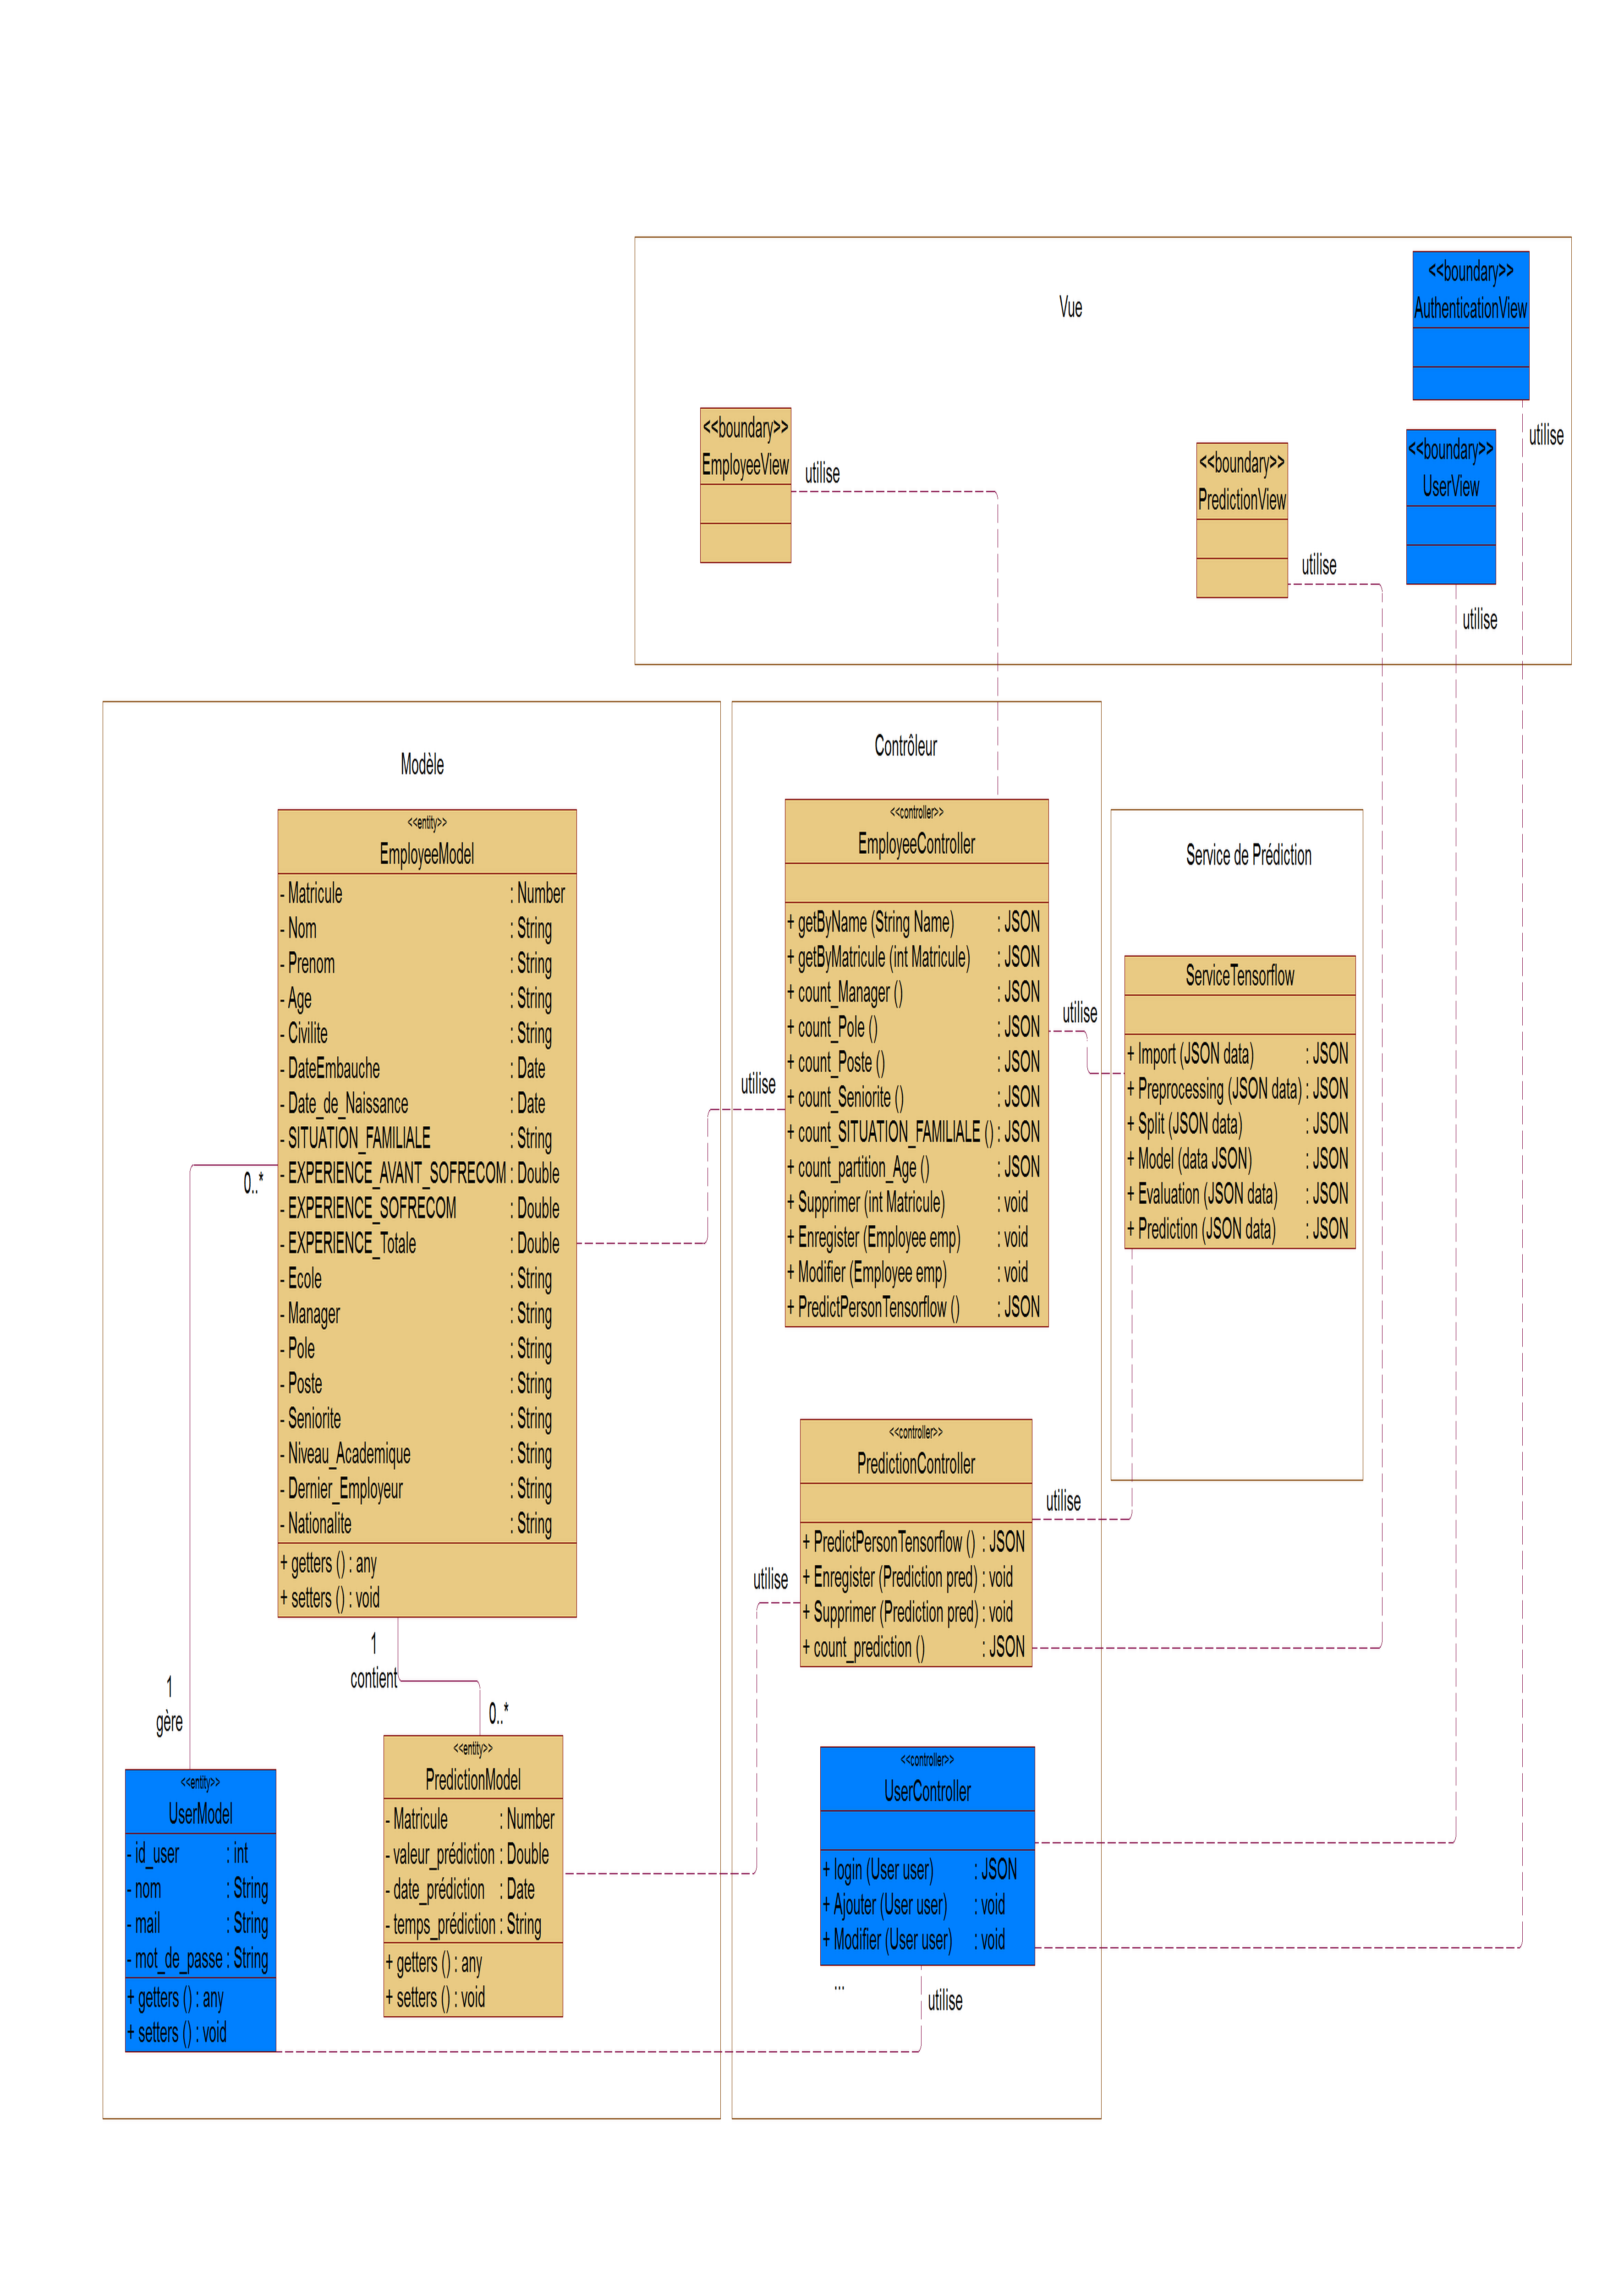
\includegraphics[width=1\linewidth]{img/diagclasse3_new_3.png}}
    \caption{Diagramme de classes}
    \label{fig:diagclasse3_new_3}
    \end{figure}
\newpage
\subsubsection{Diagrammes de séquences}

\textbf{Diagramme de séquences objet « S'authentifier »}\\
L'authentification est indispensable pour gérer l'accès des utilisateurs et la sécurité de l’application.\\
Les différentes étapes de cette fonctionnalité sont représentées dans la figure \ref{fig:seqobjetauthentifier}.
  \begin{figure}[htpb]
    \centering
    \fcolorbox{brown}{white}{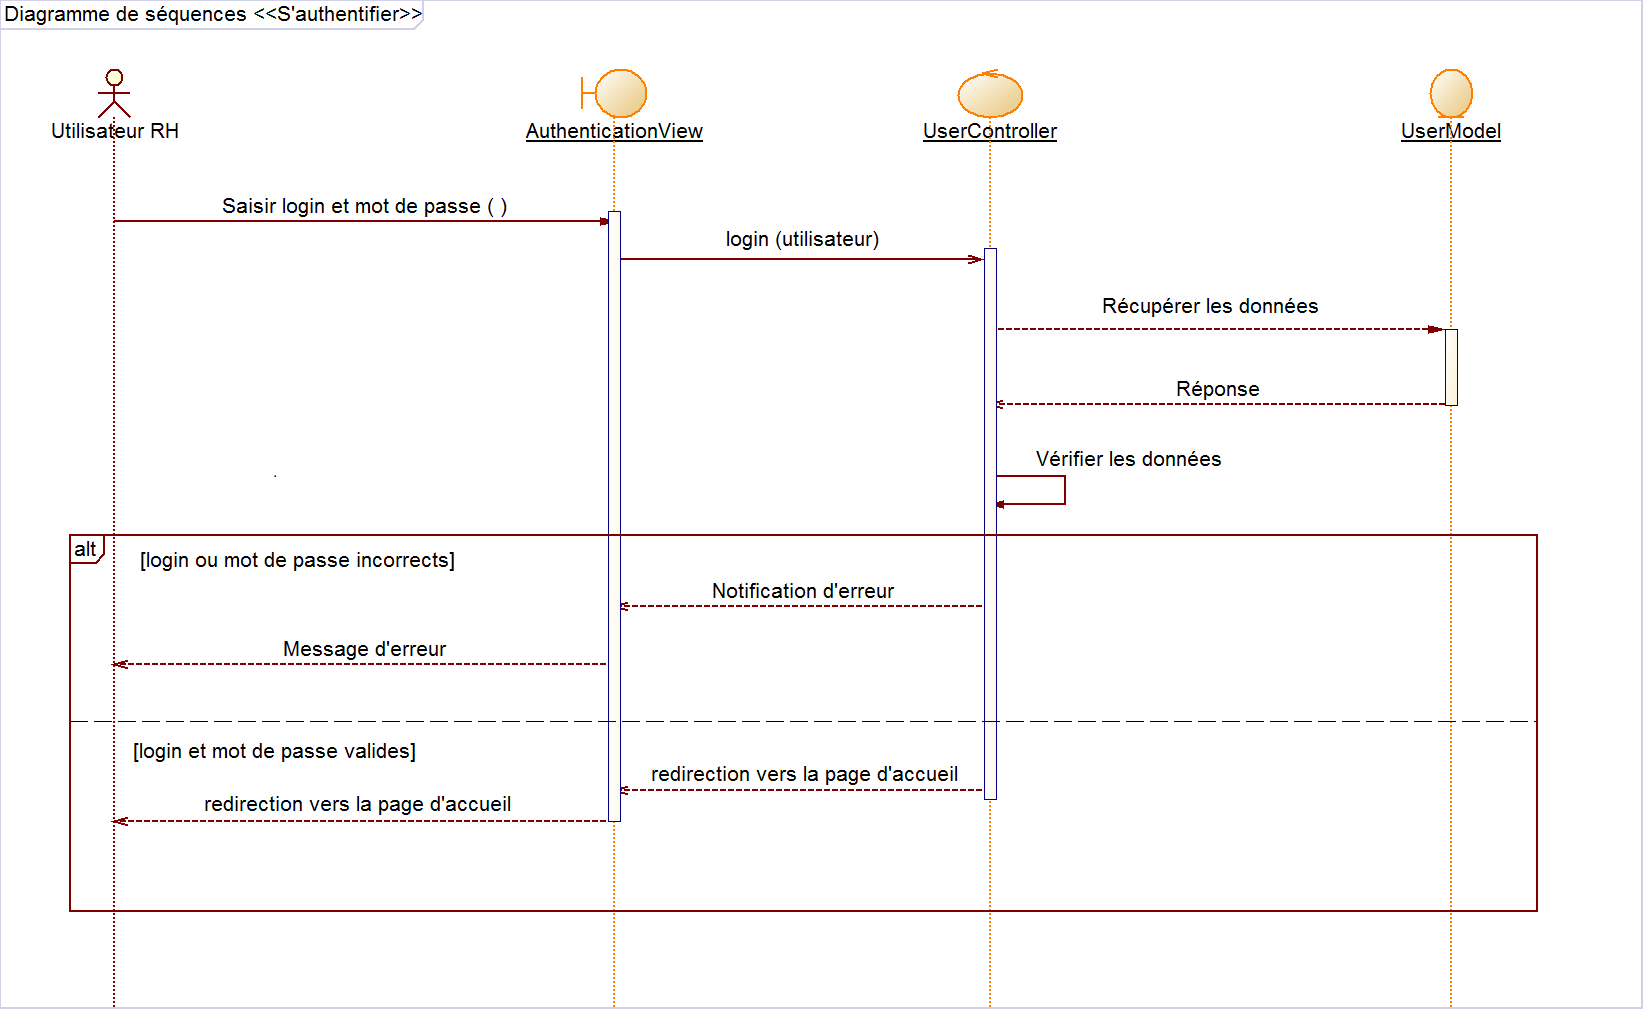
\includegraphics[width=1\linewidth]{img/seqobjetauthentification_final.png}}
    \caption{Diagramme de séquences objet « s'authentifier »}
    \label{fig:seqobjetauthentifier}
    \end{figure}
\\
\textbf{Diagramme de séquences objet « Ajouter un compte utilisateur »}\\
Chaque acteur intervenant dans l’application dispose d’un compte utilisateur. L’ajout d’un nouvel utilisateur (compte utilisateur) est assuré par l’administrateur de l’application. Ce dernier saisit les données relatives au nouvel utilisateur dans l'interface « UserView ». Une fois saisies, ces données sont prises en charge par le contrôleur « UserController » qui procède à la vérification de leur validité.\newline
Une fois ces données validées, le contrôleur ordonne la création d’un nouveau compte utilisateur dans l'entité « UserModel ». Si ce n'est pas le cas, un message d’erreur est affiché.\newline
La figure \ref{fig:diagseqobjetAjouterUtilisateur} illustre le déroulement du processus de la réalisation de cette tâche.
\newpage
 \begin{figure}[htpb]
    \centering
    \fcolorbox{brown}{white}{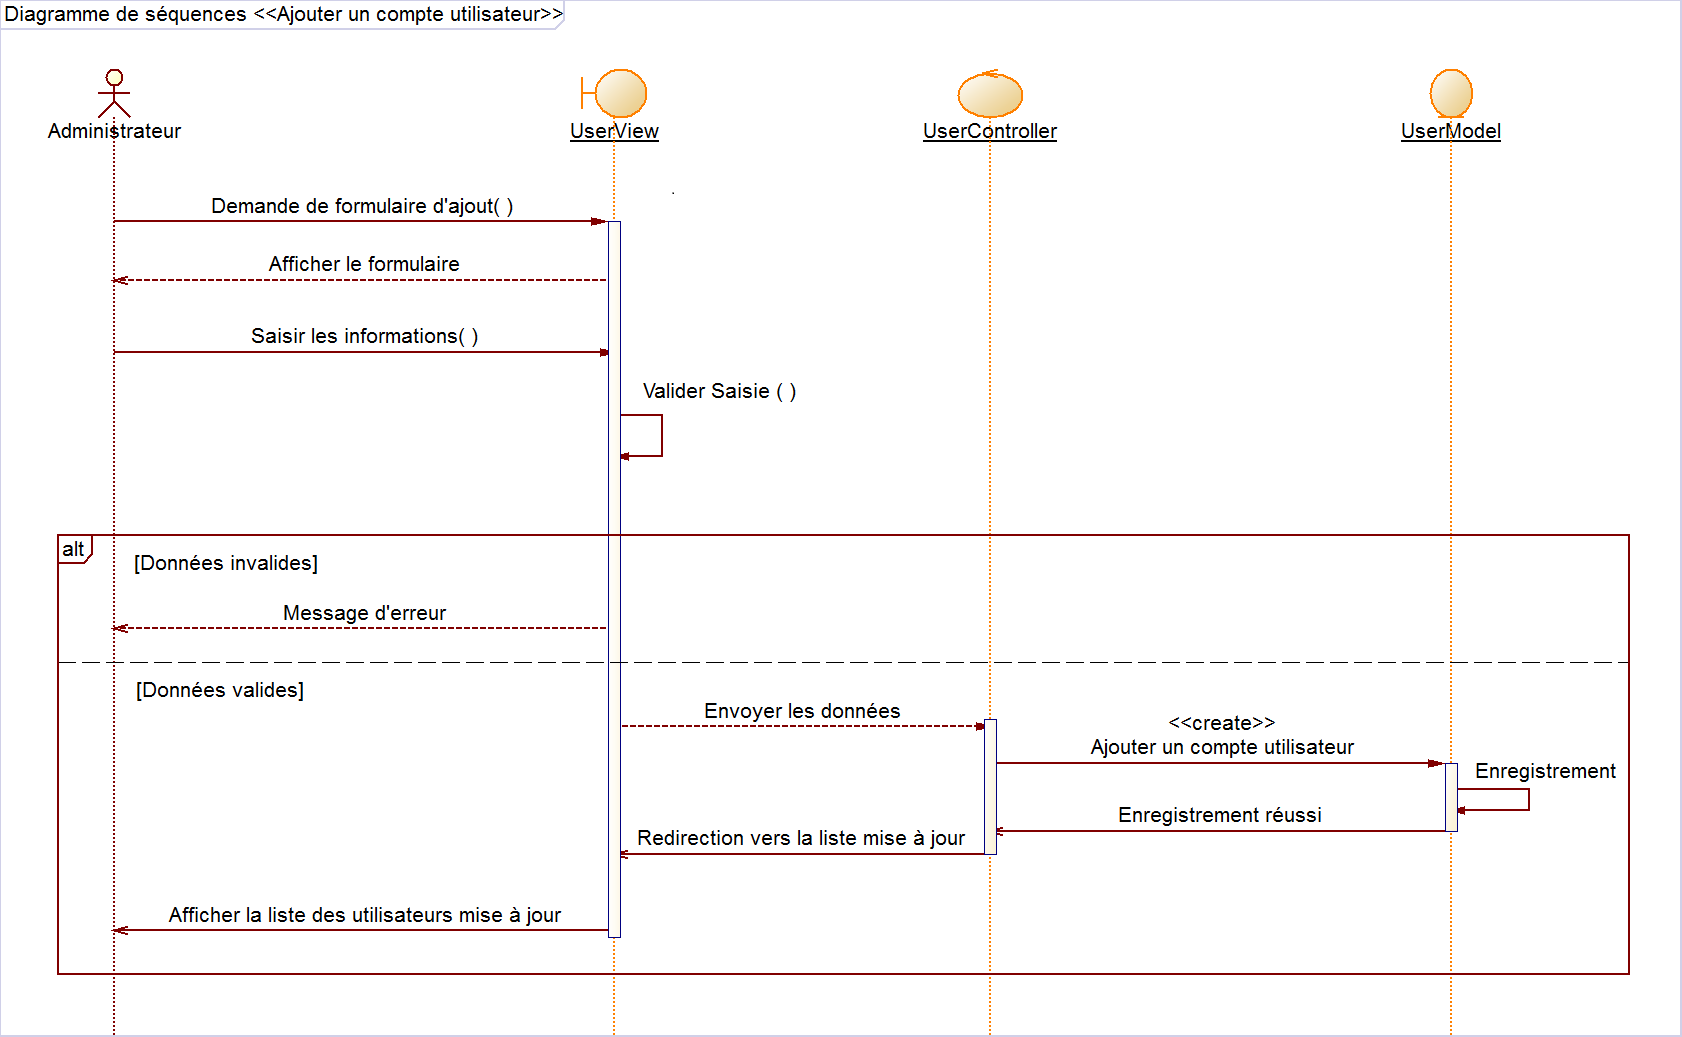
\includegraphics[width=1\linewidth]{img/diagseqobjetAjouterUtilisateur_final.png}}
    \caption{Diagramme de séquences objet « Ajouter un compte utilisateur »}
    \label{fig:diagseqobjetAjouterUtilisateur}
    \end{figure}

\textbf{Diagramme de séquences objet « Modifier un compte utilisateur »}\\
L’administrateur peut modifier des données relatives à un compte utilisateur déjà pris en charge par l’application. Il sélectionne le compte à modifier à partir de l’interface « UserView » et prend en charge les modifications à apporter.\newline Une fois le compte est choisi, le contrôleur « UserController » récupère les données, ordonne l’affichage de la page du compte à modifier par l’administrateur et ordonne la mise à jour du compte utilisateur.\newline
La figure \ref{fig:SeqObjetModifierUtilisateur} expose le déroulement du processus de la réalisation de cette tâche.
\newpage
    \begin{figure}[htpb]
    \centering
    \fcolorbox{brown}{white}{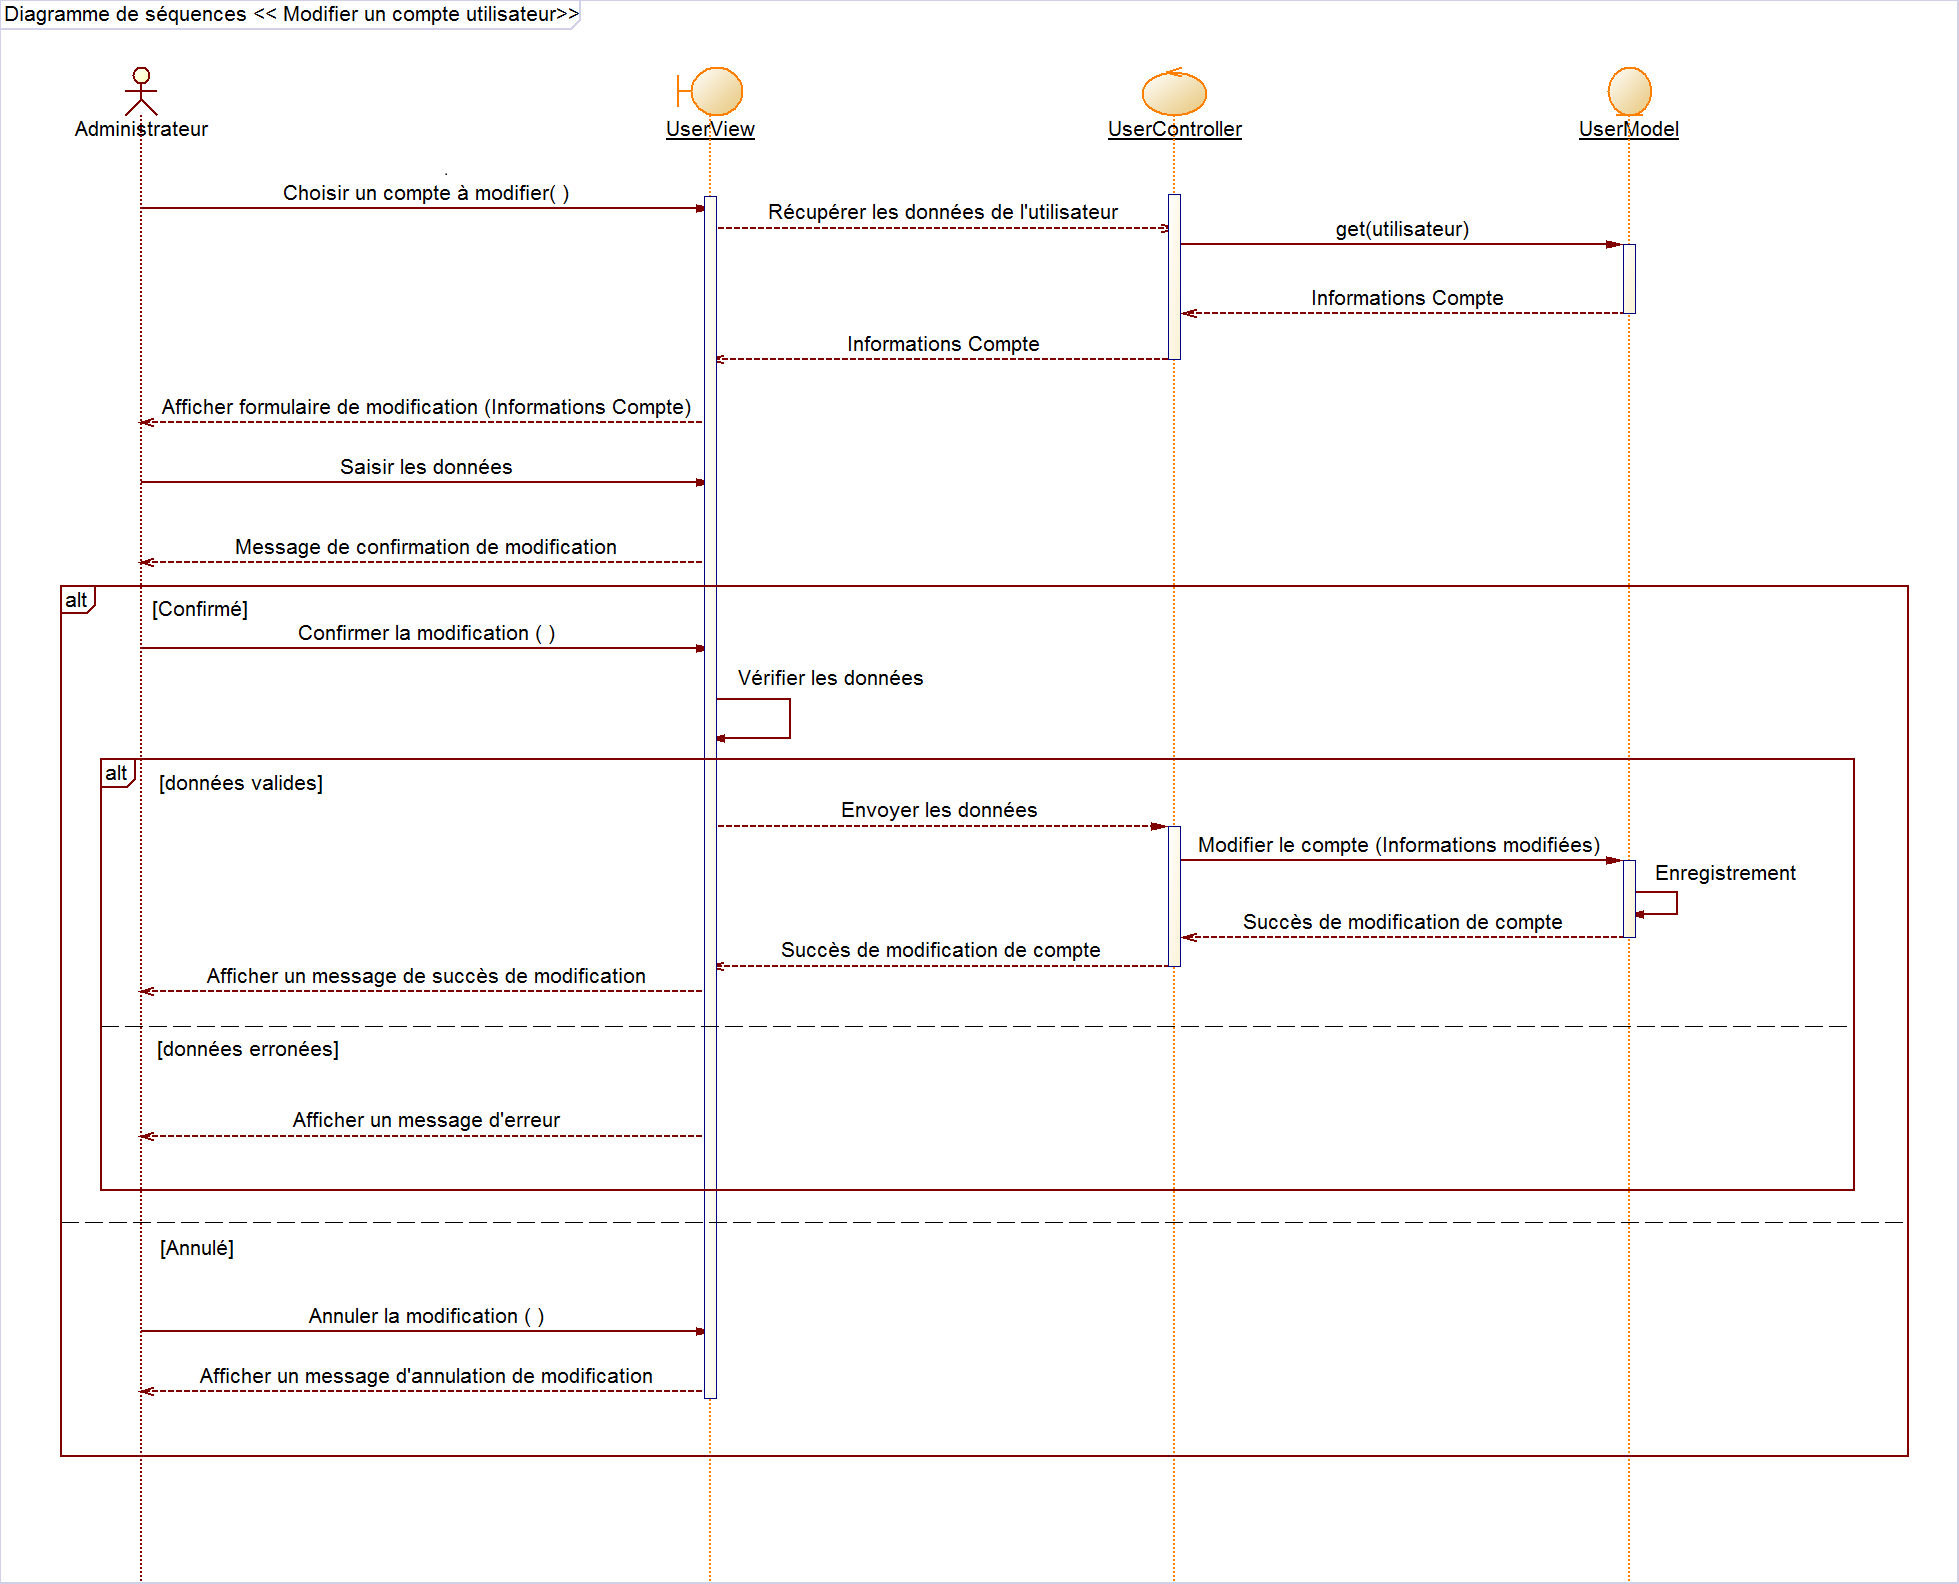
\includegraphics[width=1\linewidth]{img/SeqObjetModifierUtilisateur_final.png}}
    \caption{Diagramme de séquences objet « Modifier un compte utilisateur »}
    \label{fig:SeqObjetModifierUtilisateur}
    \end{figure}
\textbf{Diagramme de séquences objet « Supprimer un compte utilisateur »}\\
La suppression d’un compte utilisateur est à la charge de l’administrateur de l’application. Ce dernier sélectionne le compte concerné à partir de l’interface « UserView ». Une fois le compte est choisi, le contrôleur « UserController » ordonne la suppression du compte utilisateur.\newline
La suppression ne peut porter que sur un compté déjà pris en charge par l’application.\newline
La figure \ref{fig:seqobjetsupprimerUtilisateur} illustre le déroulement du processus de la réalisation de cette tâche.
\newpage
 \begin{figure}[htpb]
    \centering
    \fcolorbox{brown}{white}{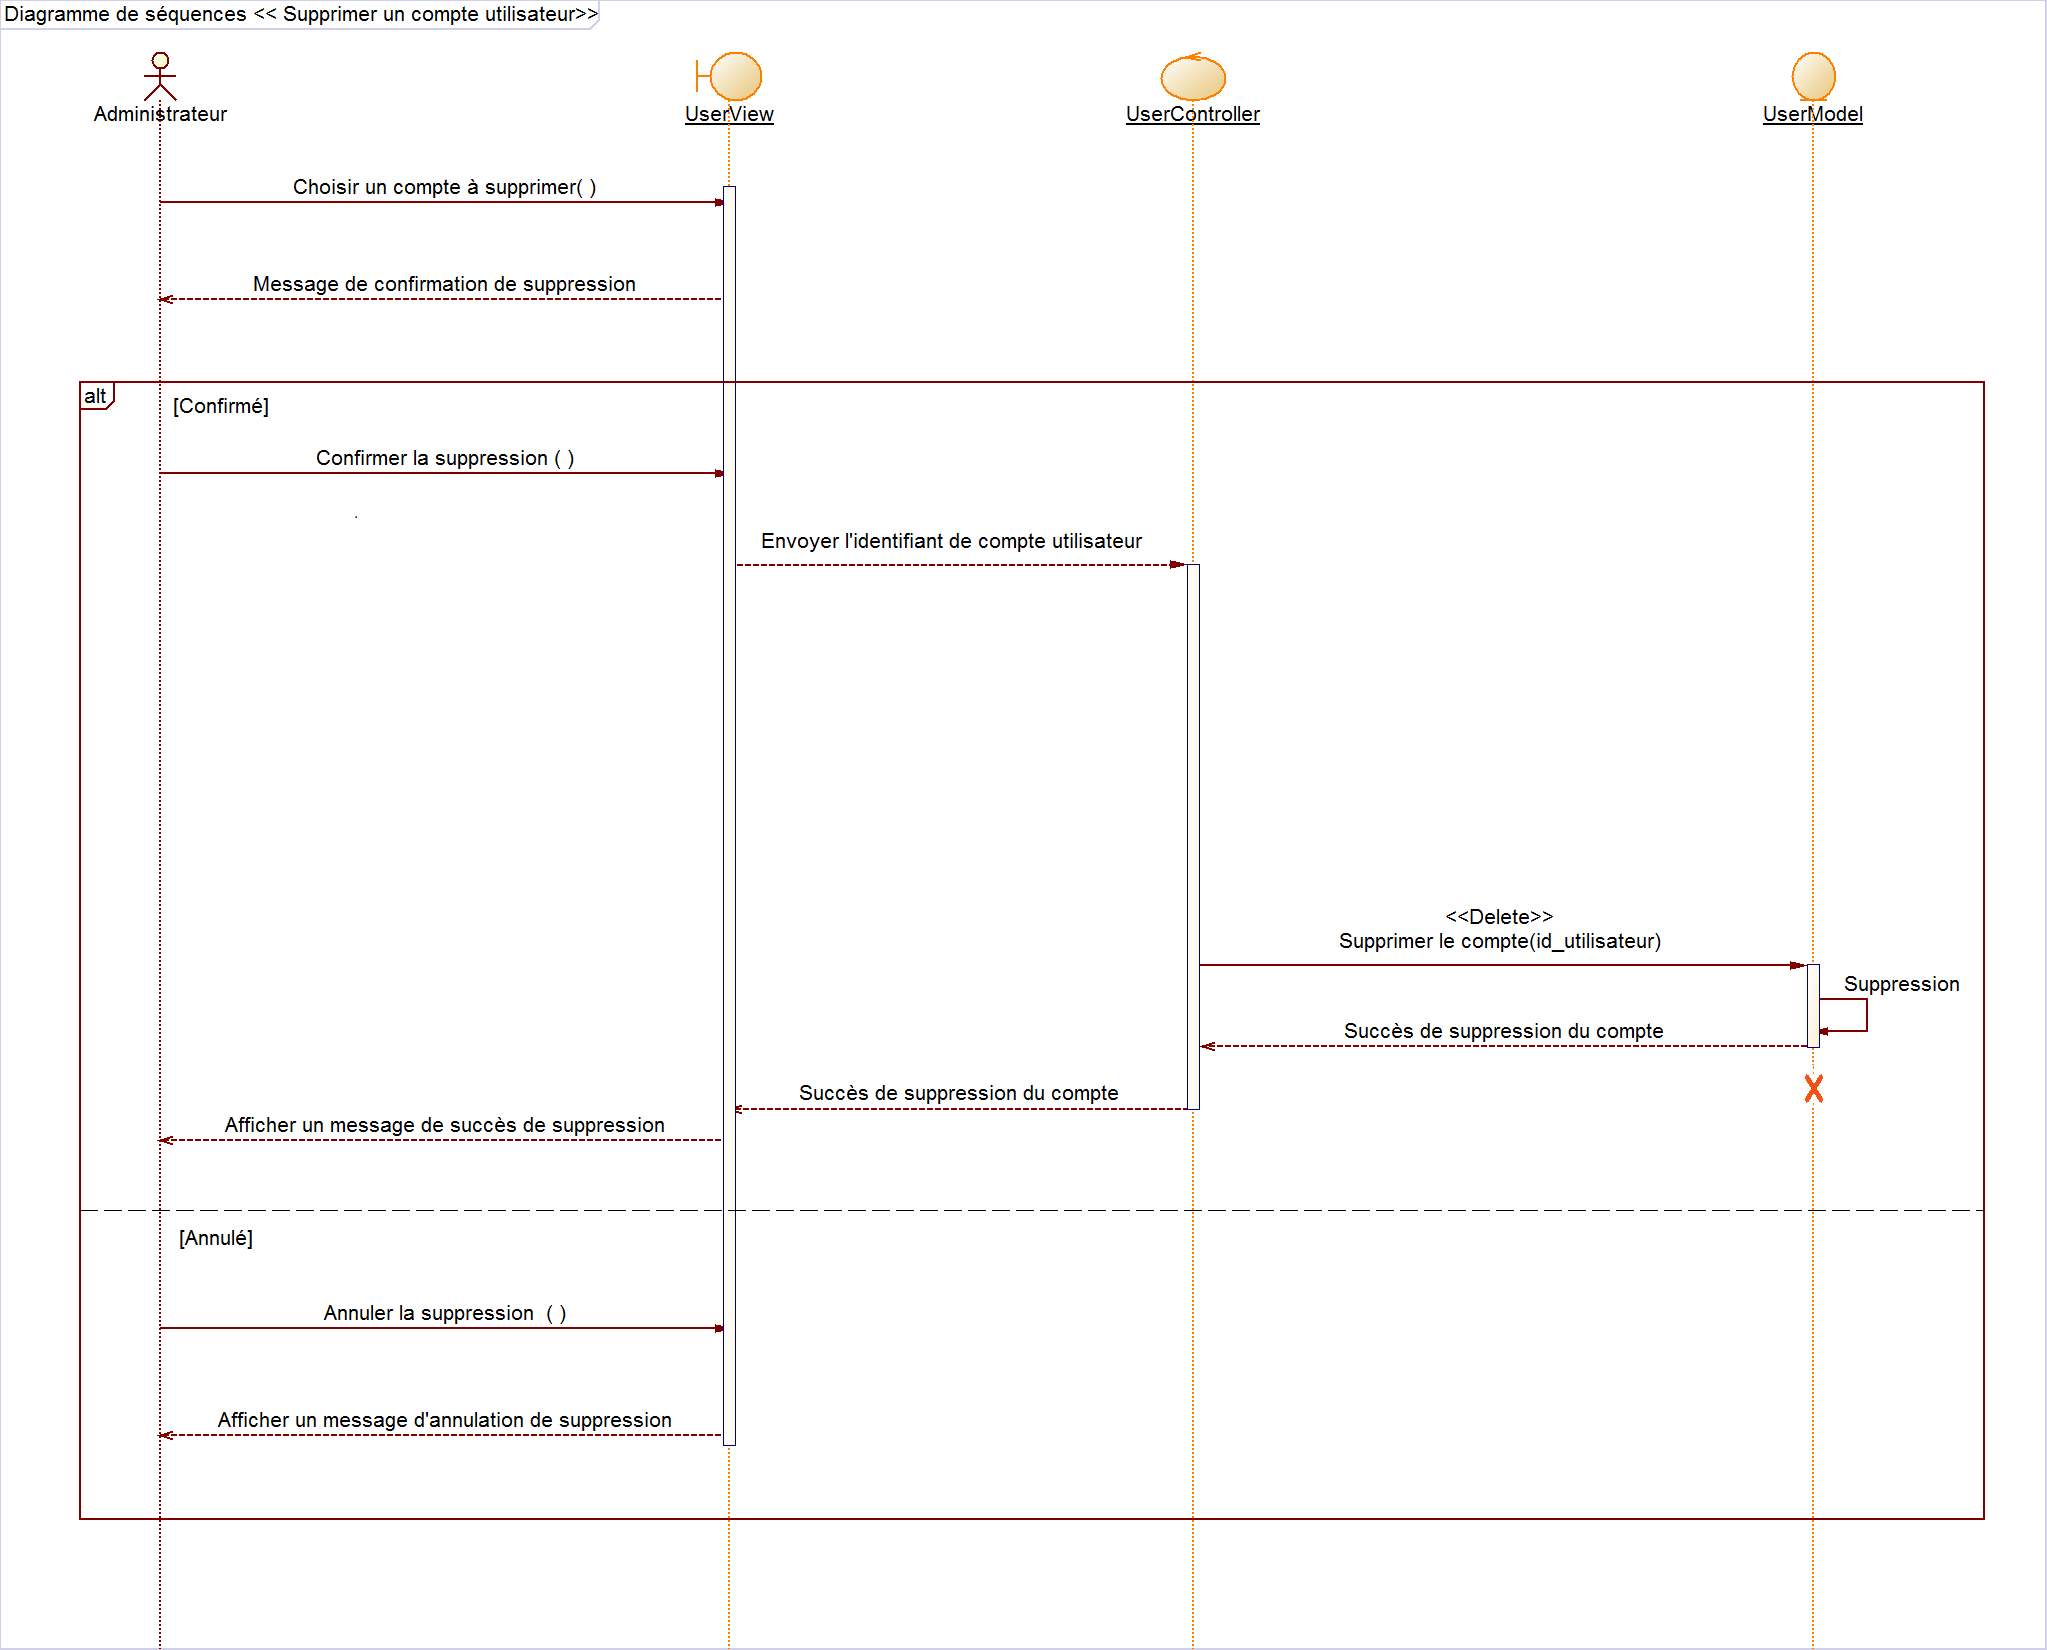
\includegraphics[width=1\linewidth]{img/seqobjetsupprimerUtilisateur_final.png}}
    \caption{Diagramme de séquences objet « Supprimer un compte utilisateur »}
    \label{fig:seqobjetsupprimerUtilisateur}
    \end{figure}



\subsection{Réalisation}
Dans cette partie, nous allons exposer les différentes interfaces de notre application réalisées dans
le troisième sprint.\newline Nous avons choisi l’administrateur comme utilisateur vu qu’il présente à travers ces interactions la majeure partie des principales fonctionnalités de ce sprint.

\textbf{Interface de l'authentification}\\
L’interface représentée dans la figure \ref{fig:authenticationInterface} permet à l’utilisateur de s’authentifier pour pouvoir accéder à l’application. L’utilisateur doit d’abord saisir son login et mot de passe.
\newpage
 \begin{figure}[htpb]
    \centering
    \fcolorbox{brown}{white}{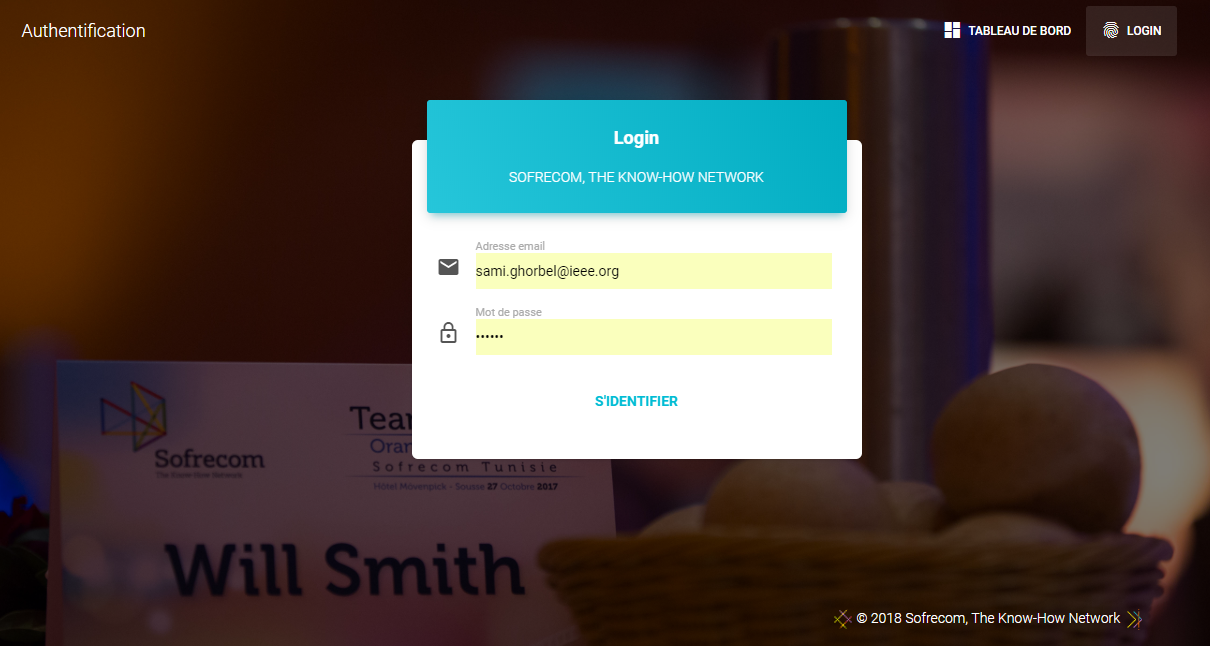
\includegraphics[width=0.93\linewidth]{img/Authentification2.png}}
    \caption{Interface de l’authentification}
    \label{fig:authenticationInterface}
    \end{figure}

\textbf{Interface de gestion des comptes utilisateurs}\\
La figure \ref{fig:crud_user} illustre la gestion des comptes utilisateurs qui interviennent dans l’application.\newline
Chaque compte utilisateur est caractérisé par:
\begin{itemize}
    \item Identifiant unique;
    \item Nom de l’utilisateur;
    \item Adresse électronique;
    \item Rôle (administrateur ou utilisateur RH).
\end{itemize}
 \begin{figure}[htpb]
    \centering
    \fcolorbox{brown}{white}{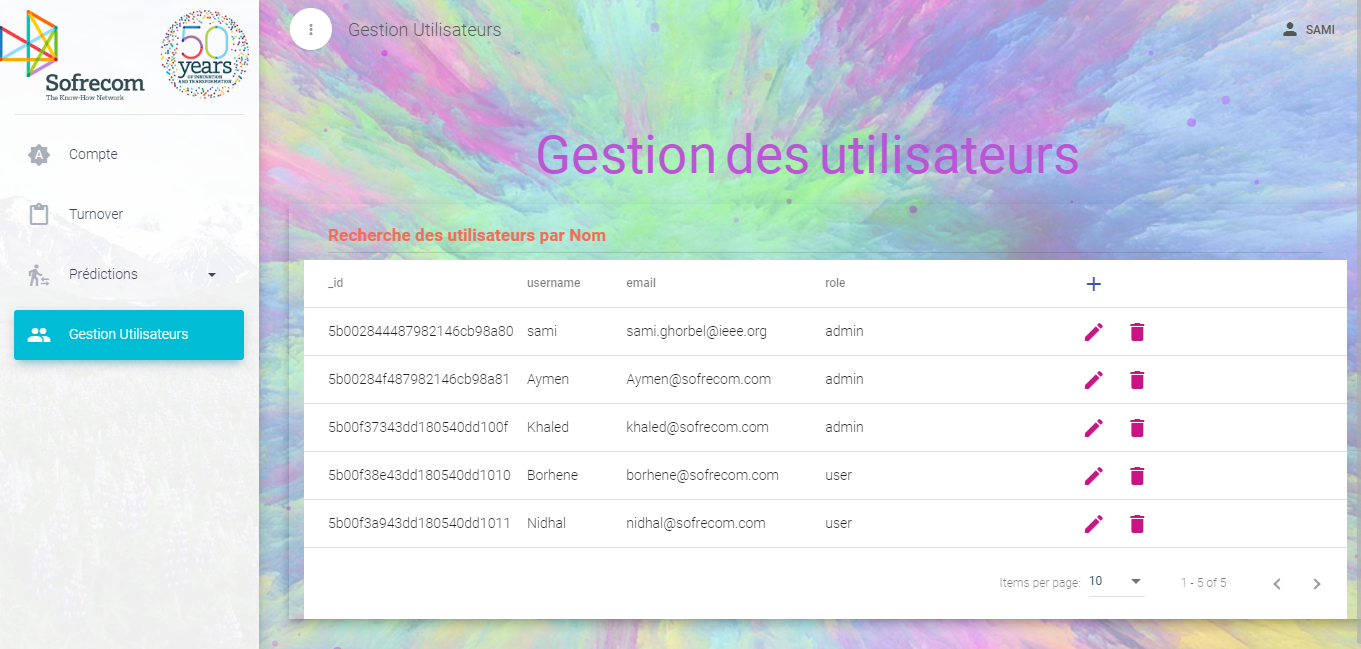
\includegraphics[width=0.93\linewidth]{img/Crud_user.png}}
    \caption{Interface de gestion des comptes utilisateurs}
    \label{fig:crud_user}
    \end{figure}
\newpage
\textbf{Interface d'ajout d’un nouveau compte utilisateur}\\
La figure \ref{fig:addUser} ci-dessous représente l’interface d’ajout d’un nouveau compte utilisateur.
 \begin{figure}[htpb]
    \centering
    \fcolorbox{brown}{white}{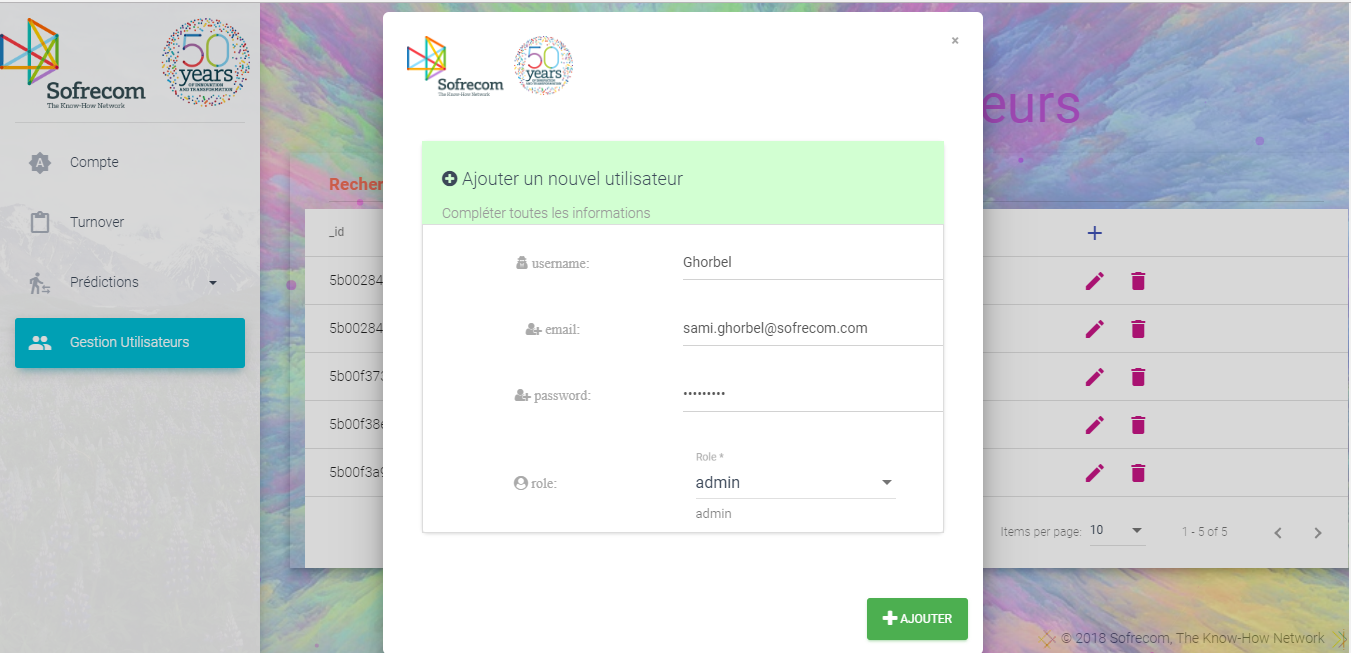
\includegraphics[width=1\linewidth]{img/addUser.png}}
    \caption{Interface d'ajout d'un compte utilisateur}
    \label{fig:addUser}
    \end{figure}
\newline
\textbf{Interface de modification des informations d’un compte utilisateur}\\
Comme illustré par la figure \ref{fig:updateuser}, l’administrateur peut modifier les informations d'un compte utilisateur choisi.
\begin{figure}[htpb]
    \centering
    \fcolorbox{brown}{white}{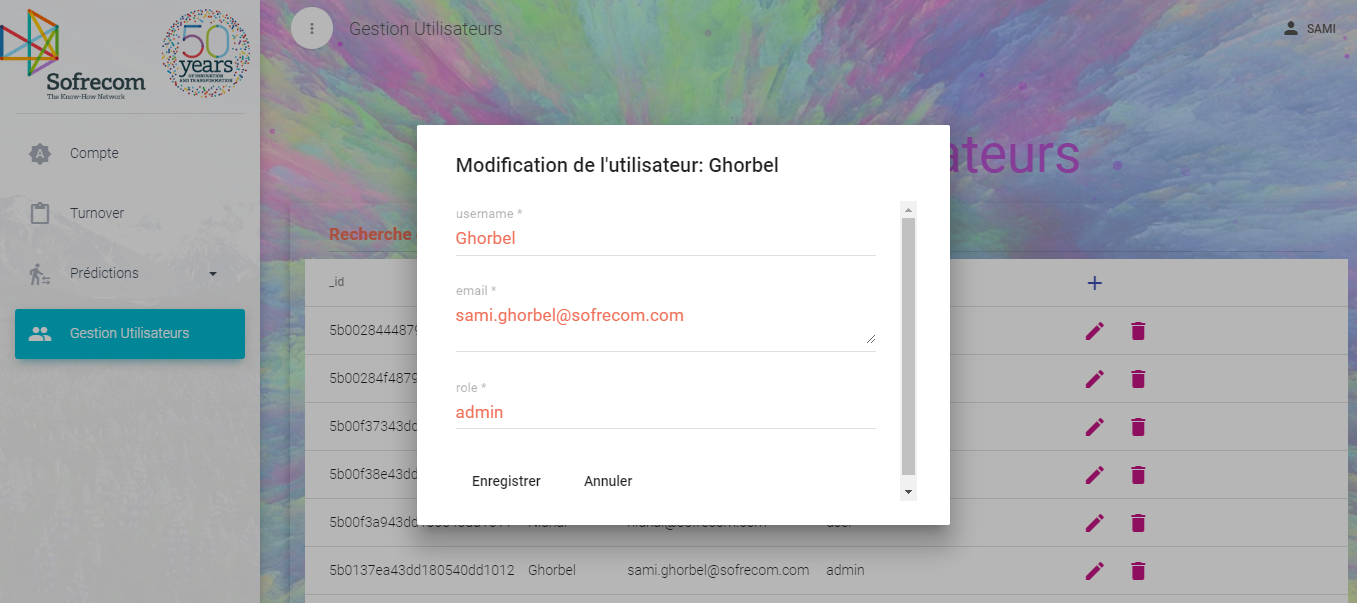
\includegraphics[width=1\linewidth]{img/updateuser.png}}
    \caption{Interface de modification des informations d’un compte utilisateur}
    \label{fig:updateuser}
    \end{figure}
\newpage
\textbf{Interface de suppression d’un compte utilisateur}\\
L'administrateur choisit un compte utilisateur à supprimer. Une alerte de confirmation sera déclenchée pour confirmer la suppression du compte concerné comme indiqué sur la figure \ref{fig:deleteUser}.
\begin{figure}[htpb]
    \centering
    \fcolorbox{brown}{white}{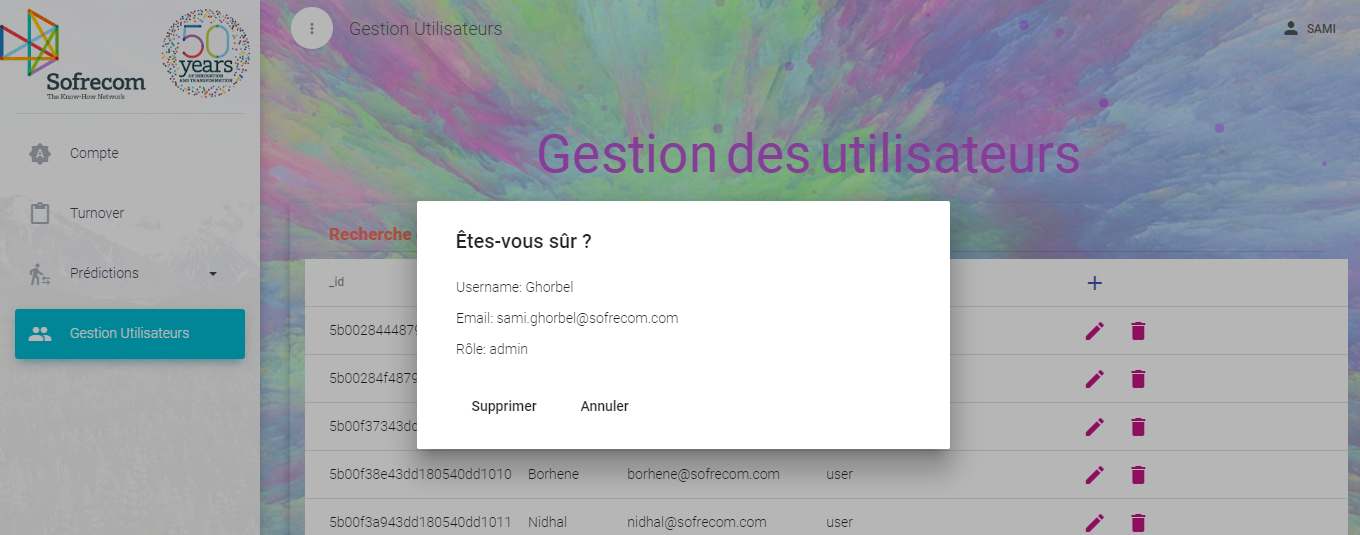
\includegraphics[width=1\linewidth]{img/deleteUser.png}}
    \caption{Interface de suppression d’un compte utilisateur}
    \label{fig:deleteUser}
    \end{figure}

\textbf{Interface de succès de suppression d’un compte utilisateur}\\
Dès que l’administrateur confirme la suppression du compte utilisateur, une alerte de succès sera affichée
comme le montre la figure \ref{fig:successdeleteUser}.
\begin{figure}[htpb]
    \centering
    \fcolorbox{brown}{white}{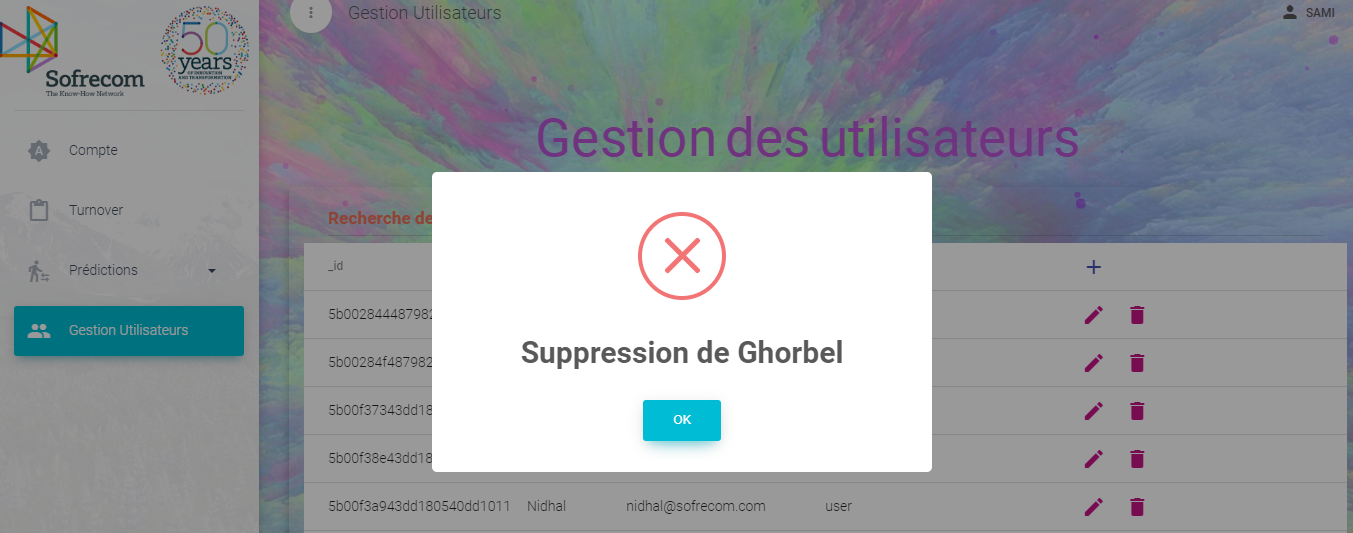
\includegraphics[width=1\linewidth]{img/successdeleteUser.png}}
    \caption{Interface de succès de suppression d’un compte utilisateur}
    \label{fig:successdeleteUser}
    \end{figure}
\subsubsection{Test et validation}
Nous avons rassemblé dans le tableau 5.6 un ensemble de scénarios de cas de tests fonctionnels associés au sprint 3.
\newpage
\captionof{table}{Tests fonctionnels du sprint 3}

\begin{tabular}{@{}| >{\raggedright}p{.25\textwidth}|>{\raggedright} p{5.1 cm}|>{\raggedright}p{5.2 cm}| >{\centering\arraybackslash}p{.10\textwidth}|@{}}
\hline \rowcolor{lightgray} \hspace{1.5pc} \textbf{Cas de test}  & \hspace{1.5pc}  \textbf {Démarches} & \hspace{0.5pc}  \textbf {Comportement attendu} &   \textbf {Résultat} \\

\hline  S’authentifier & Demander la page\newline
d’authentification.\newline
Saisir et valider le login et le mot de
passe.
& Affichage de la page d’authentification.\newline
Redirection vers la page d’accueil.


& Conforme \\

\hline   Ajouter un compte utilisateur & Demander la page de gestion des utilisateurs.\newline
Remplir et valider le formulaire d'ajout.
& Affichage de la page de gestion des utilisateurs.\newline
Ajout effectué.


& Conforme \\

\hline  Modifier un compte utilisateur & Demander la page de gestion des utilisateurs.\newline
Cliquer sur modifier..\newline\newline
Saisir et valider le formulaire
de modification.
& Affichage de la page de gestion des utilisateurs.\newline
Affichage de formulaire de
modification.\newline
Modification effectuée.


& Conforme \\


\hline  Supprimer un compte utilisateur & Demander la page de gestion des utilisateurs.\newline
Cliquer sur supprimer.\newline\newline
Confirmer la suppression.
& Affichage de la page de gestion des utilisateurs.\newline
Affichage d'un message de confirmation de suppression.\newline
Suppression effectuée.


& Conforme \\

\hline

\end{tabular}
\newline
\\
Après avoir vérifié le bon fonctionnement du code et des fonctionnalités, le troisième livrable a été testé et validé par le Product Owner.

\section{Sprint 4 Visualisation du tableau de bord}
\subsection{Spécification fonctionnelle}
\subsubsection{Backlog du Sprint}
\subsubsection{Diagrammes de cas d’utilisations détaillés du sprint 4}
\subsection{Conception}
   \subsubsection{Diagrammes de séquences}
\subsection{Réalisation}
\subsubsection{Test et validation}

   
   
\section*{Conclusion}
